
\documentclass{standalone}
\usepackage{tikz}
\usetikzlibrary{positioning, calc, matrix, arrows.meta}
\tikzset{
    every matrix/.style={matrix of math nodes},hp/.style={column 3/.style={anchor={base east}}},Hp/.style={column 4/.style={anchor={base east}}},>=Stealth
}

\begin{document}  
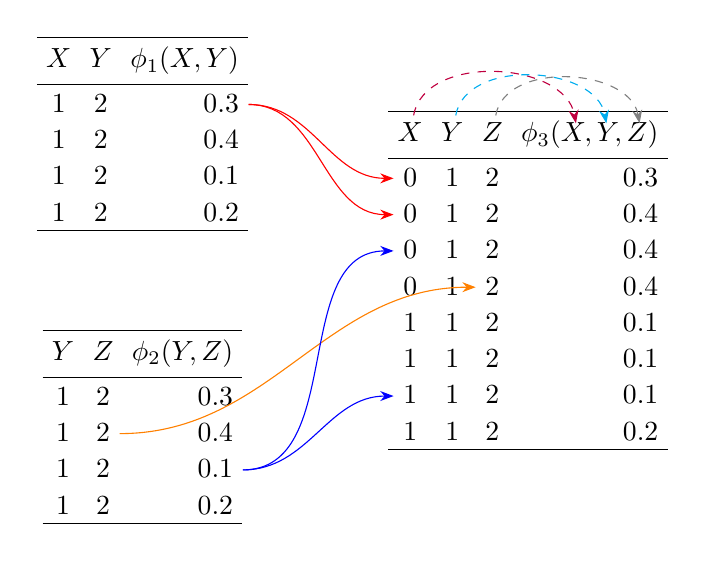
\begin{tikzpicture}

\matrix [hp] (a) { \hline
X & Y &  \phi _1(X,Y) \\ \hline
1 & 2 & 0.3 \\
1 & 2 & 0.4 \\
1 & 2 & 0.1 \\
1 & 2 & 0.2 \\ \hline \\
};

\matrix[below = of a, hp] (b) { \hline
Y & Z & \phi _2(Y,Z) \\ \hline
1 & 2 & 0.3 \\
1 & 2 & 0.4 \\
1 & 2 & 0.1 \\
1 & 2 & 0.2 \\ \hline \\
};

\coordinate (x) at ($(a)!0.5!(b)$);
\matrix[right = 3cm of x, Hp] (c) { \hline
X & Y & Z & \phi _3(X,Y,Z) \\ \hline
0 & 1 & 2 & 0.3 \\
0 & 1 & 2 & 0.4 \\
0 & 1 & 2 & 0.4 \\
0 & 1 & 2 & 0.4 \\
1 & 1 & 2 & 0.1 \\
1 & 1 & 2 & 0.1 \\
1 & 1 & 2 & 0.1 \\
1 & 1 & 2 & 0.2 \\ \hline \\
};

\draw[->, red] (a-2-3) to[in=180, out=0] (c-2-1);
\draw[->, red] (a-2-3) to[in=180, out=0] (c-3-1);

\draw[->, orange] (b-3-2) to[in=180, out=0] (c-5-3);

\draw[->, blue] (b-4-3) to[in=180, out=0] (c-4-1);
\draw[->, blue] (b-4-3) to[in=180, out=0] (c-8-1);

\draw[->, purple, dashed] (c-1-1) to[in=100, out=80] ([xshift=-0.5em, yshift=0.5em]c-1-4);
\draw[->, cyan, dashed] (c-1-2) to[in=100, out=80] ([xshift=0.6em, yshift=0.5em]c-1-4);
\draw[->, gray, dashed] (c-1-3) to[in=100, out=80] ([xshift=1.8em, yshift=0.5em]c-1-4);

\end{tikzpicture}
\end{document}